The aim of the code portion of this assignment is to implement a Red-Black Tree
which can store paired ``finish number'' and ``VPN'' values. The Red-Black Tree
is required to sort the pairs by finish number. In order to ensure that the code
is working as intended, 100 input pairs must be inserted to the tree, with the
original input pairs and the tree following all insertions being printed to
verify its operation.

Provided for the purposes of the coding section of this assignment were a
selection of random number generating functions, along with an implementation of
a red-black tree\cite{zentut} which needs to be modified. The red-black tree
implementation
takes integer values for its elements, however, the output from the random
number generator is of type long. The required implementation must also be able
to perform insertions of two values.

In order to store both the ``finish key'' and the ``vpn'' values, a C structure
named ``node\_entry'' was defined in the ``node\_entry.h'' file. In this header
file, the finish key is defined as an unsigned long, while the vpn is defined as
an unsigned int. A function to display the values of the struct is defined
within this header file, and is implemented within the ``node\_entry.c'' file.

\begin{figure}[H]
	\centering
	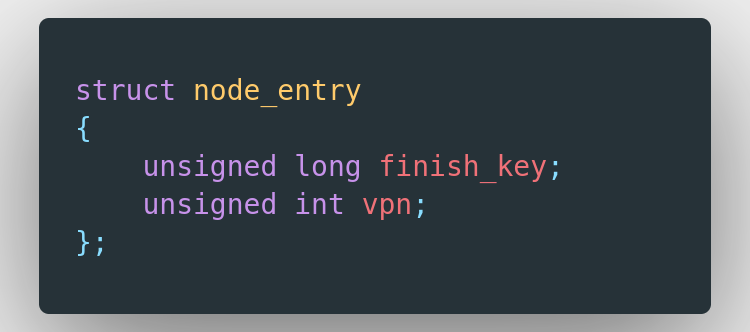
\includegraphics[width=0.8\textwidth]{images/nodeEntry}
	\caption{Node Entry Structure}
	\label{fig:images-nodeEntry}
\end{figure}

Within the ``redblack.h'' file, the type definition for ``ElementType'' must be
changed from type int to type ``struct node\_entry''. This allows for the finish
key/vpn pairs to be passed in as arguements to the functions of the red-black
tree, such as insertion etc.

\begin{figure}[H]
	\centering
	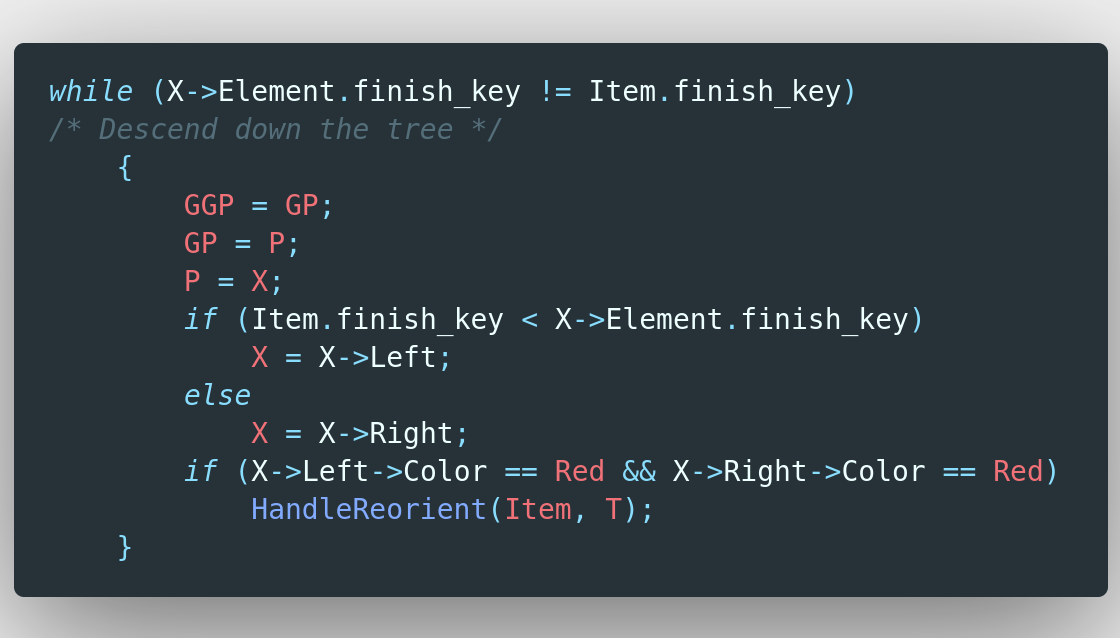
\includegraphics[width=0.8\textwidth]{images/example}
	\caption{Example of Modifications to the Red-Black Tree Code}
	\label{fig:images-ex}
\end{figure}

Within the ``redblack.c'' file, all references to ``Element'', which is the
value in the tree, must be replaced with ``Element.finish\_key''. This allows
for all sorting within the tree to be done based on the finish key, rather than
on the vpn. The return type of the ``Retrieve'' function must also be changed to
``long'', as it is no longer returning an integer value, rather the value of the
finish key, which is long.

Within the main function, the tree and random number generator are both
initialized. The tree is initialized as an empty red-black tree, and the random
number generator is initialised with the seeds (0, 0, 1541, 0402). Within the
``init'' function, the seeds are set to (1, 2, 3, 4). An empty array of type
node\_entry is defined, with a size of 100. A loop iterates from 0 to
100, populating the finish key values with random long values from 0-999, using
the ``fairdie'' function. The vpn values are populated with the iteration value,
i.e. 0-99. Within this loop, each new node\_entry item is inserted into the tree
using the ``Insert'' function. The ``PrintTree'' function is then used in order
to print the sorted contents of the tree, which verifies the correct operation
of the tree.
